
\subsection{Analyse ING}
Die Analyse der ING hat ergeben, dass weniger Fehler auftreten als bei der Sparkasse. Die Startseite weist keine Fehler auf. Die Unterseiten, wie die Login-Seite, weisen aber doch Fehler auf. Einige davon sind auch über die Seiten hinweg inkonsistent.

So sind die Social Media Icons auf der Startseite noch korrekt mit einem Label versehen, während auf der Login-Seite kein Label mehr angegeben ist. Die folgende Abbildung 4.4 zeigt das HTML der Social Media Icons auf der Startseite. 

\begin{figure}[H]
    
\includegraphics[width=\textwidth]{img/ing_sm-accessible-name.png}
    \caption{Social Media Icons mit Label}
\end{figure}

Im Vergleich dazu steht die Abbildung 4.5 der Login-Seite, in der kein Label mehr angegeben ist.

\begin{figure}[H]
    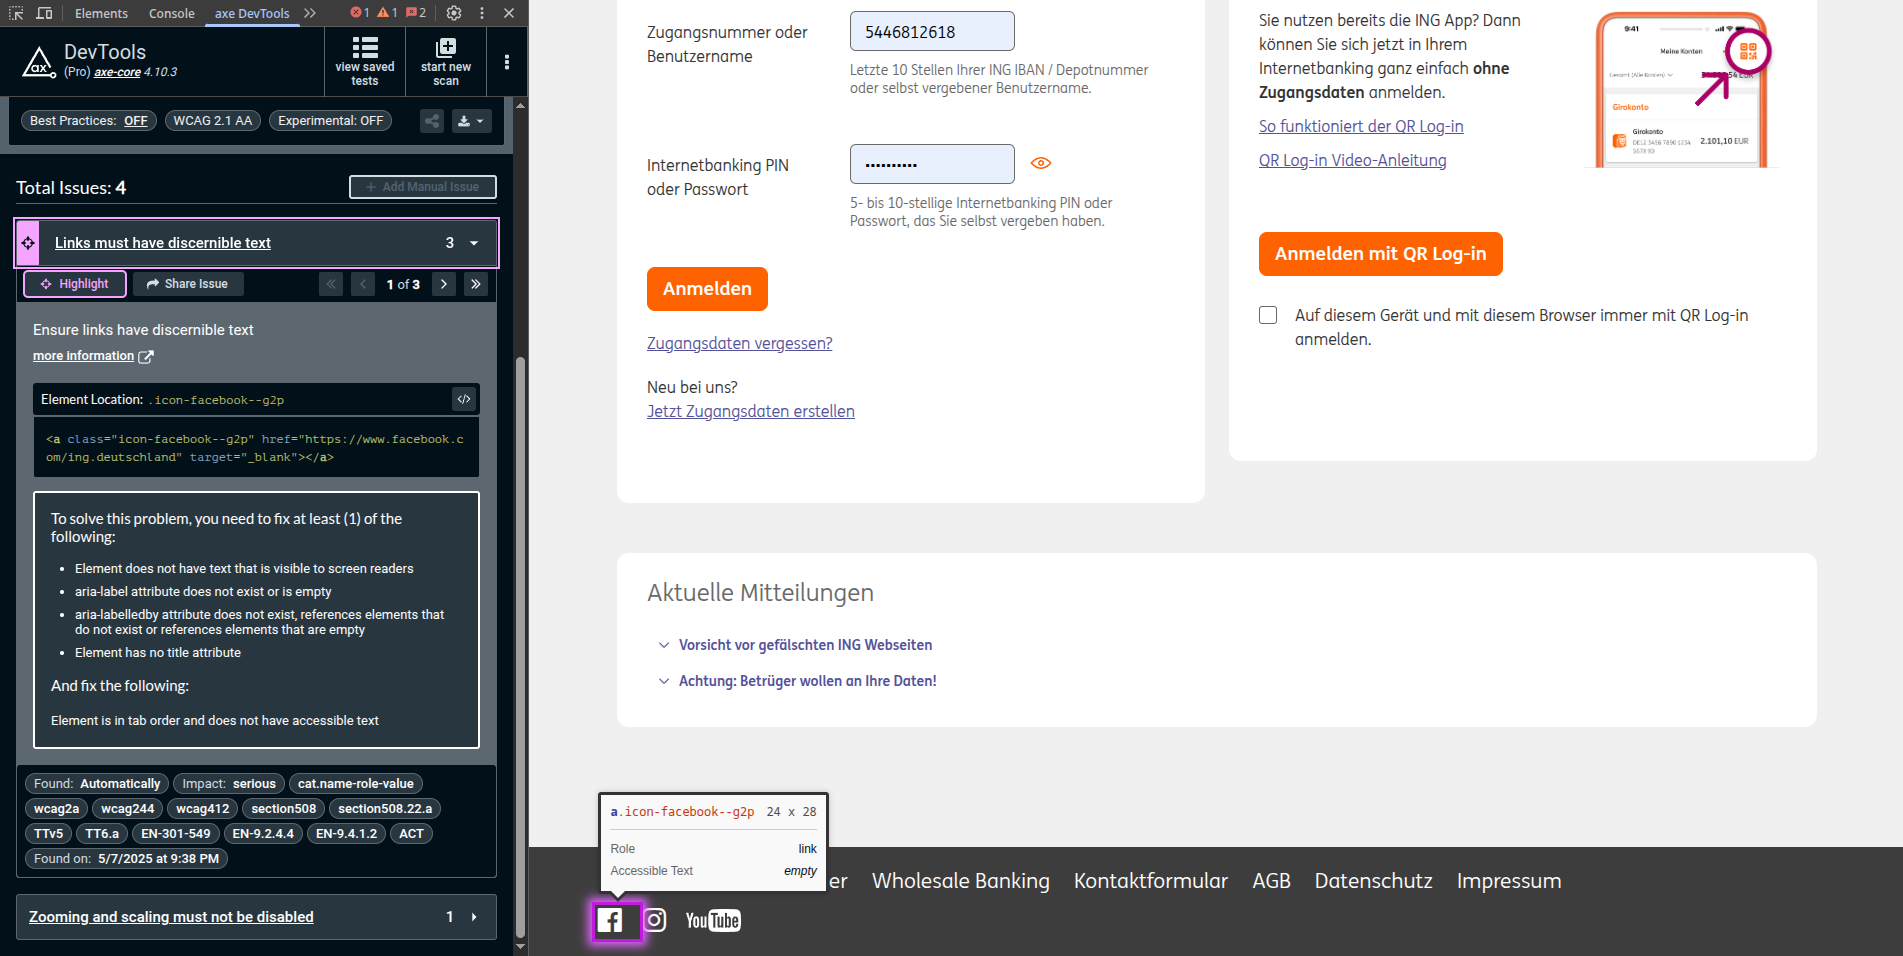
\includegraphics[width=\textwidth]{img/ing_login_sm-no-accessible-name.png}
    \caption{Social Media Icons ohne Label}
\end{figure}

Zusätzlich wurde das Scaling mit user-scalable=no ausgeschaltet. Zu sehen in Abbildung 4.6.

\begin{figure}[H]
\begin{lstlisting}[language=html]
<meta name="viewport" 
    content="width=device-width,
    initial-scale=1,
    maximum-scale=1,
    minimum-scale=1,
    user-scalable=no"
    >
\end{lstlisting}
\caption{Scaling mit user-scalable=no}
\end{figure}

Die Anzahl der Fehler ist auf die drei getesteten Seiten aber überschaubar und die Startseite ist mit keinem Fehler ein gutes Beispiel für eine Barrierefreie Umsetzung. 

Im Vergleich zur Sparkasse überscheiden sich die Fehler zum größten Teil. Bis auf den Scaling-Fehler betreffen die Fehler, die gefunden wurden, auch die Sparkasse. Dazu gehören die korrekte Verwendung von Aria-Atrributen, das Verständnis von dem Zweck eines Links und die richtige Semantik vom HTML. 

\begin{figure}[H]
\begin{tikzpicture}
\begin{axis}[
    width=\textwidth,
    height=10cm,
    ybar,
    bar width=12pt,
    xlabel={WCAG-Kriterium},
    ylabel={Fehleranzahl},
    symbolic x coords={ 9.1.3.1, 9.1.4.4, 9.2.4.4, 9.4.1.2 },
    xtick=data,
    x tick label style={rotate=45, anchor=east},
    ymin=0,
    ymax=300,
    enlarge x limits=0.1,
    legend style={cells={anchor=west}, legend pos=north east},
    nodes near coords,
    nodes near coords style={font=\scriptsize},
]
\addplot table[x=WCAG-Kriterium,y=Fehleranzahl_axe,col sep=tab] {csv/output/wcag_analyse_ing_xxxx.csv};
\addplot table[x=WCAG-Kriterium,y=Fehleranzahl_WAVE,col sep=tab] {csv/output/wcag_analyse_ing_xxxx.csv};
\legend{axe,WAVE}
\end{axis}
\end{tikzpicture}
\caption{Auswertung Analyse ING}
\end{figure}